\documentclass{beamer}
\usetheme{Frankfurt}
\usepackage[utf8]{inputenc}
\usepackage{charter}
\usepackage{tikz}
\usepackage{graphicx}
\usepackage{amsmath}
\usepackage{amssymb}
\usepackage{listings}
\beamertemplatenavigationsymbolsempty

%% Title slide formatting %%

\pgfdeclareimage[width=\paperwidth]{titlebackground}{Images/title-slide-background.png}
\setbeamerfont{subtitle}{size=\tiny}
\setbeamertemplate{endpage}{
	\begin{picture}(0,0)
		\scalebox{1.01}{
		\put(-28.5,-163){%
			\pgfuseimage{titlebackground}
		}
		}
		\put(0,-115){%
			\begin{minipage}[b][4.5cm][t]{0.5\textwidth}
				\color{white}
				\usebeamerfont{title}
				{\textbf{Thank Your} \\ \textbf{For You Attention !}}
			\end{minipage}
		}
	\end{picture}
}
\setbeamertemplate{title page}{
	\begin{picture}(0,0)
		\scalebox{1.01}{
			\put(-28.5,-163){%
				\pgfuseimage{titlebackground}
			}
		}
		\put(0,-75){%
			\begin{minipage}[b][4.5cm][t]{0.5\textwidth}
				\color{white}
				\usebeamerfont{title}
				{\inserttitle\\[0.9cm]}
				\usebeamerfont{subtitle}
				{\insertauthor\par}
				{\insertinstitute\\[0.3cm]}
				{\insertdate}
			\end{minipage}
		}
	\end{picture}
}


%% General slide formatting %%

\definecolor{oxfordblue}{RGB}{4,30,66}

\pgfdeclareimage[width=0.9cm]{oxfordlogo}{Images/oxford-logo.png}
\pgfdeclareimage[width=1cm]{mathslogo}{Images/mathematics-logo.png}
\pgfdeclareimage[width=0.9cm]{pizzalogo}{Images/pizza-logo.png}

\setbeamertemplate{headline}
{%
	\begin{picture}(0,0)
		\put(314,-50){%
			\pgfuseimage{oxfordlogo}
		}
		\put(20,-55){%
			\rule{320pt}{0.4pt}
		}
	\end{picture}
}

\setbeamertemplate{frametitle}
{%
	\begin{picture}(0,0)
		\put(-8,-20){%
			\normalsize\textbf{\color{oxfordblue}\insertframetitle}
		}
		\put(-7,-25){%
			\small\color{oxfordblue}\insertframesubtitle
		}
	\end{picture}
}

\setbeamertemplate{footline}
{%
	\begin{picture}(0,0)
		\put(20,30){%
			\rule{320pt}{0.4pt}
		}
		\put(20,14){%
			\pgfuseimage{mathslogo}
		}
		\put(100,14){%
			\color{oxfordblue}\insertshortdate
		}
		\put(160,14){%
			\color{oxfordblue}\insertshorttitle
		}
		\put(337,14){%
			\color{oxfordblue}\insertpagenumber
		}
	\end{picture}%
}
\setbeamercolor{block title}{bg=oxfordblue!30,fg=black}

\definecolor{codegreen}{rgb}{0,0.6,0}
\definecolor{codegray}{rgb}{0.5,0.5,0.5}
\definecolor{codepurple}{rgb}{0.58,0,0.82}
\definecolor{backcolour}{rgb}{0.95,0.95,0.92}

\lstdefinestyle{mystyle}{
	%backgroundcolor=\color{backcolour},   
	commentstyle=\color{codegray},
	keywordstyle=\color{oxfordblue},
	numberstyle=\tiny\color{codegray},
	stringstyle=\color{codegreen},
	basicstyle=\ttfamily\footnotesize,
	breakatwhitespace=false,         
	breaklines=true,                 
	captionpos=b,                    
	keepspaces=true,                 
	numbers=left,                    
	numbersep=5pt,                  
	showspaces=false,                
	showstringspaces=false,
	showtabs=false,                  
	tabsize=2
}

\lstset{style=mystyle}

%% Information (author, title, etc.) %%

\title[Netgen Meets Firedrake]{Netgen Meets Firedrake} % short title for footer
\author%
{%
	\sc{P. E. Farrell} *, \sc{S. Zampini}$\;\dagger$, \underline{\sc{U. Zerbinati}} *\\
}
\institute%
{%
	* \textit{Mathematical Institute}\\
	\;\textit{University of Oxford}\\
	\\
	$\;\dagger\;$\textit{Extreme Computing Research Center}\\
	\;\textit{King Abdullah University of Science and Technology}
}

\date[Firedrake 2023]{Firedrake User Meeting, Exeter, 6th of January 2023} % short date for footer



%% Content of slides %%

\begin{document}
	\begin{frame}[plain]
		\titlepage
	\end{frame}
	%
	\begin{frame}
		\frametitle{Solving a Partial Differential Equation}
		\begin{minipage}{0.75\textwidth}
			When solving a partial differential equation the following macro steps can be identified:
			$\newline$
			\begin{itemize}
				\item[\color{oxfordblue}$\blacktriangleright$] Geometrical modelling,
				\item[\color{oxfordblue}$\blacktriangleright$] Meshing,
				\item[\color{purple}$\blacktriangleright$] Discretising a PDE,
				\item[\color{purple}$\blacktriangleright$] Solving the linear or nonlinear system.
			\end{itemize}
			We aim to allow the Firedrake user to do all the steps above described in a single script.
		\end{minipage}
		\begin{minipage}{0.2\textwidth}
			\vspace{-0.3cm}
			\begin{figure}
				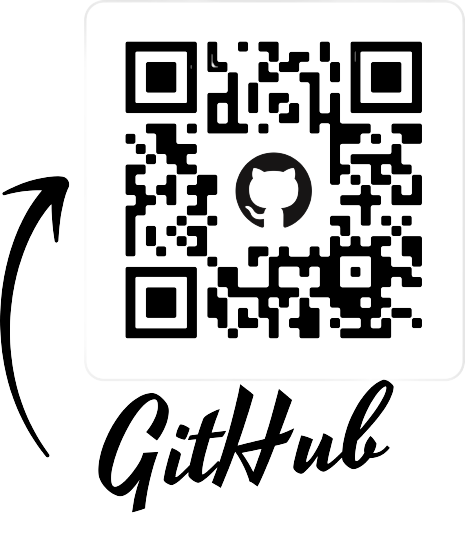
\includegraphics[scale=0.2]{Figures/QR}
			\end{figure}
		\end{minipage}
	\end{frame}
	\begin{frame}
		\frametitle{Why NetGen?}
		\framesubtitle{}
		NetGen is an advancing front 2D/3D-mesh generator, with many interesting features. Among the most important:
		$\newline$
		\begin{itemize}
			\item[\color{oxfordblue}$\blacktriangleright$] Python wrapping (through pybind11),
			\item[\color{oxfordblue}$\blacktriangleright$] Multiple ways of describing the geometry to be meshed, i.e. its builtin \textbf{Constructive Solid Geometry} (\textbf{CSG}) and the \textbf{Open Cascade Technology} (\textbf{OCCT}) geometry kernel,
			\item[\color{oxfordblue}$\blacktriangleright$] Supports mesh refinement (also anisotropic mesh refinement).
		\end{itemize}
	\end{frame}
	\begin{frame}
		\frametitle{Getting Started -- Installing NetGen}
			\begin{block}{Install NetGen using Firedrake scripts}
				\begin{center}
				\lstinline! python3 firedrake-install --netgen !
				\\
				\lstinline! python3 firedrake-update --netgen !
				\end{center}
			\end{block}
			\begin{alertblock}{PETSc}
				If you are using an external PETSc installation, it should be updated to include commit \texttt{654059db}.
			\end{alertblock}
			\begin{alertblock}{NetGen}
				If installing from scratch, use the NetGen fork from the Firdrake project GitHub.
			\end{alertblock}
	\end{frame}
	\begin{frame}
		\frametitle{Getting Started -- Unstructed Mesh}
		$\newline$
		\lstinputlisting[language=Python,firstline=2]{Codes/Poisson2DMesh.py}
	\end{frame}
	\begin{frame}
		\frametitle{Getting Started -- Unstructed Mesh}
		\begin{figure}
			\centering
			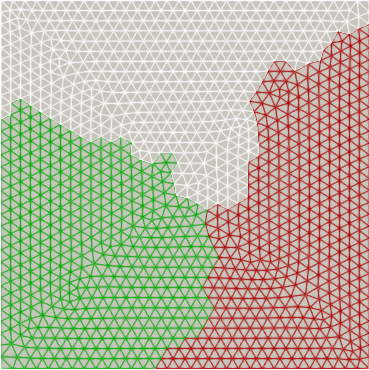
\includegraphics[scale=0.23]{Figures/ParallelMesh}
			\qquad
			\qquad
			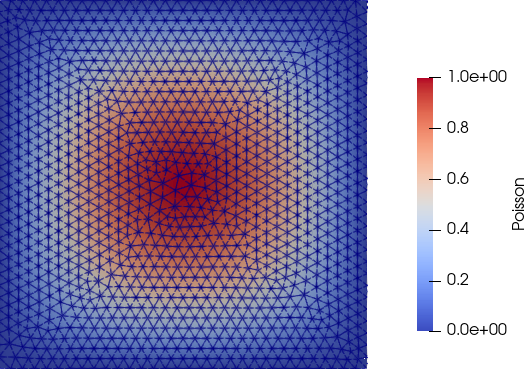
\includegraphics[scale=0.23]{Figures/Poisson2D}
		\end{figure}
	\end{frame}
	\begin{frame}
		\frametitle{Getting Started -- CSG 2D}
		$\newline$
		\lstinputlisting[language=Python]{Codes/CSG2DMesh.py}
	\end{frame}
	\begin{frame}
		\frametitle{Getting Started -- CSG 2D}
		\begin{figure}
			\centering
			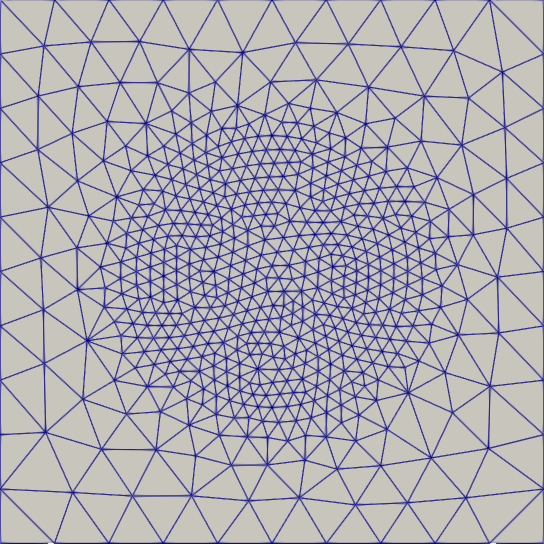
\includegraphics[scale=0.18]{Figures/CSG2DMesh}
			\begin{alertblock}{Material Identifiers}
				The material identifier specified above are carried to the DMPLEX as CELL\_SETS\_LABEL.
			\end{alertblock}
		\end{figure}
	\end{frame}
	\begin{frame}
		\frametitle{Getting Started -- CSG 3D}
		\begin{minipage}{0.7\textwidth}
			$\newline$
			\lstinputlisting[language=Python]{Codes/CSG3DMesh.py}
		\end{minipage}
		\begin{minipage}{0.25\textwidth}
			\vspace{-0.3cm}
			\begin{figure}
				\centering
				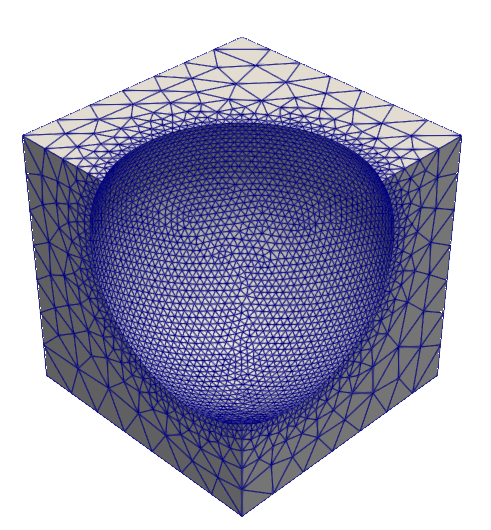
\includegraphics[scale=0.2]{Figures/CSG3DMesh}
			\end{figure}
		\end{minipage}
	\end{frame}
	\begin{frame}
			\frametitle{The Open Cascade Technology Kernel}
			$\newline$
			\begin{itemize}
				\item[\color{oxfordblue}$\blacktriangleright$] Basic OCCT objects can be used in NetGen such as: \texttt{Box}, \texttt{Cylinder}, \texttt{Point}, \texttt{Segment} and \texttt{ArcOfCircle}.
				\item[\color{oxfordblue}$\blacktriangleright$] The \texttt{fuse}, \texttt{cut} and \texttt{common} operations between OCCT objects have been wrapped in NetGen.
				\item [\color{oxfordblue}$\blacktriangleright$] Transformation operations such as \texttt{Move} and \texttt{Rotate} have also been wrapped into NetGen.
			\end{itemize}
	\end{frame}
	\begin{frame}
		\frametitle{The Open Cascade Technology Kernel}
		$\newline$
		\lstinputlisting[language=Python]{Codes/OCCGettingStarted.py}
	\end{frame}
	\begin{frame}
		\frametitle{The Open Cascade Technology Kernel}
		\begin{figure}
			\centering
			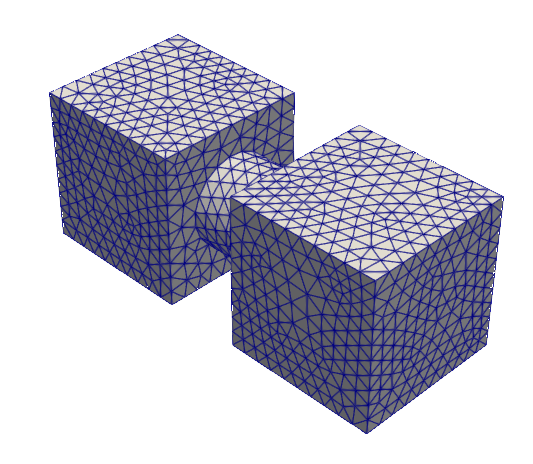
\includegraphics[scale=0.28]{Figures/OCC}
		\end{figure}
	\end{frame}
	\begin{frame}
		\frametitle{The OCCT Kernel -- The Flask Example: I}
		\begin{minipage}{0.75\textwidth}
			$\newline$
			\lstinputlisting[language=Python,firstline=1, lastline=15]{Codes/OCCBottle.py}
		\end{minipage}
		\begin{minipage}{0.15\textwidth}
			\vspace{-0.3cm}
			\begin{figure}
				\centering
				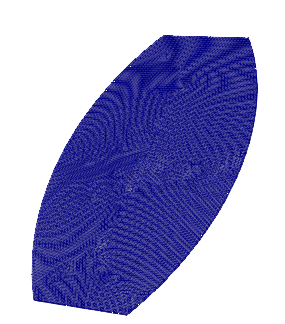
\includegraphics[scale=0.2]{Figures/OCCBottleBase}
			\end{figure}
		\end{minipage}
	\end{frame}
	\begin{frame}
		\frametitle{The OCCT Kernel -- The Flask Example: II}
		\begin{minipage}{0.65\textwidth}
			$\newline$
			\lstinputlisting[language=Python,firstline=16, lastline=27]{Codes/OCCBottle.py}
		\end{minipage}
		\begin{minipage}{0.25\textwidth}
			\vspace{-0.3cm}
			\begin{figure}
				\centering
				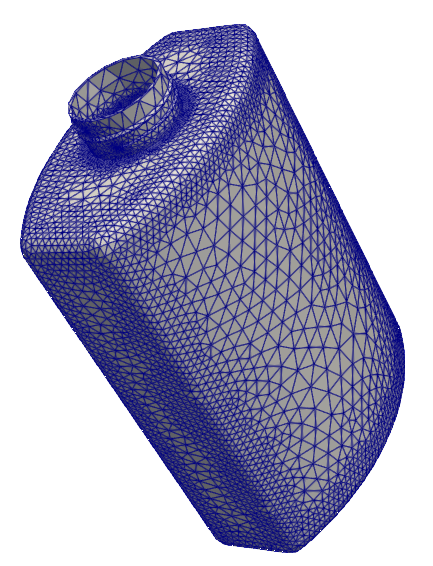
\includegraphics[scale=0.25]{Figures/OCCBottle}
			\end{figure}
		\end{minipage}
	\end{frame}
	\begin{frame}
		\frametitle{The OCCT Kernel -- Linear Elasticity: I}
		$\newline$
		\lstinputlisting[language=Python,firstline=0, lastline=14]{Codes/OCCSolid.py}
	\end{frame}
	\begin{frame}
		\frametitle{The OCCT Kernel -- Linear Elasticity: II}
		$\newline$
		\lstinputlisting[language=Python,firstline=15, lastline=29]{Codes/OCCSolid.py}
	\end{frame}
	\begin{frame}
		\frametitle{The OCCT Kernel -- Linear Elasticity: III}
		$\newline$
		\begin{figure}
			\centering
			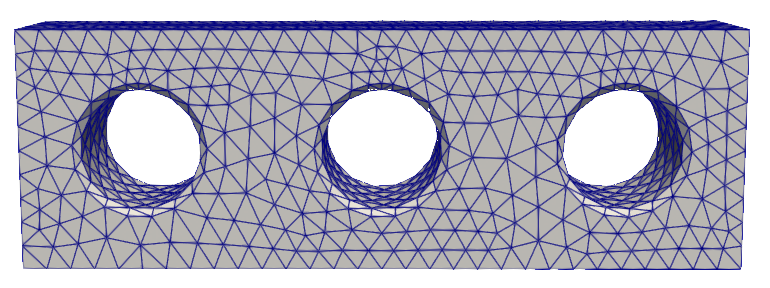
\includegraphics[scale=0.19]{Figures/OCCSolidMesh}
			\\
			\vspace{1cm}
			\qquad\qquad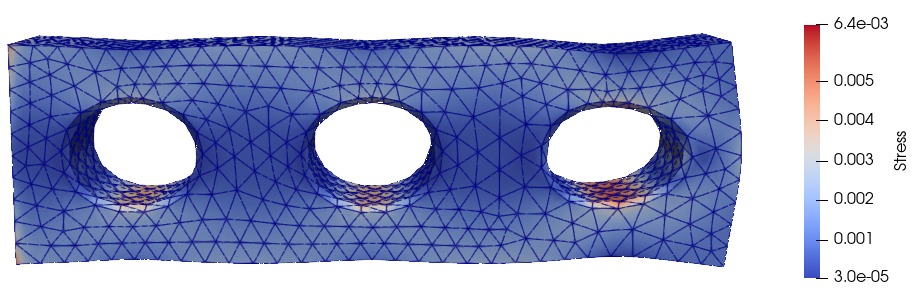
\includegraphics[scale=0.2]{Figures/OCCSolid}
		\end{figure}
	\end{frame}
	\begin{frame}
		\frametitle{The OCCT Kernel -- Multigrid: I}
		$\newline$
		\lstinputlisting[language=Python,firstline=2,lastline=17]{Codes/Multigrid.py}
	\end{frame}
	\begin{frame}
		\frametitle{The OCCT Kernel -- Multigrid: II}
		\begin{minipage}{0.8\textwidth}
			$\newline$
			\lstinputlisting[language=Python,firstline=18,lastline=29]{Codes/Multigrid.py}
		\end{minipage}
		\begin{minipage}{0.1\textwidth}
			\vspace{-0.3cm}
			\begin{figure}
				\centering
				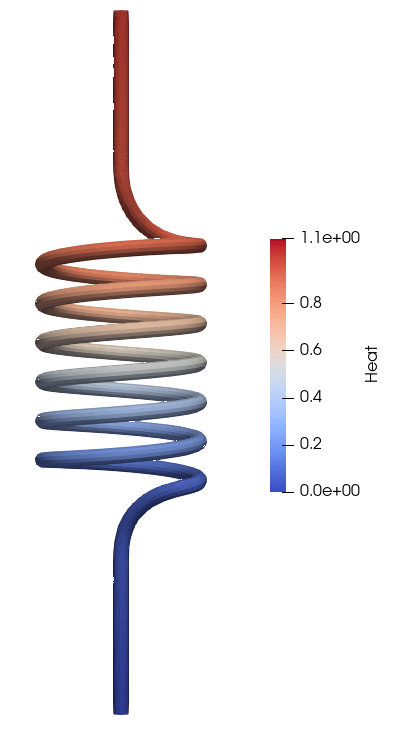
\includegraphics[scale=0.2]{Figures/Coil}
			\end{figure}
		\end{minipage}
	\end{frame}
	\begin{frame}
		\frametitle{Mesh Refinement -- Adaptive Mesh Refinement: I}
		\begin{minipage}{0.75\textwidth}
			$\newline$
			\lstinputlisting[language=Python,firstline=78, lastline=91]{Codes/PacmanV2.py}
		\end{minipage}
		\begin{minipage}{0.15\textwidth}
			\vspace{-0.3cm}
			\begin{figure}
				\centering
				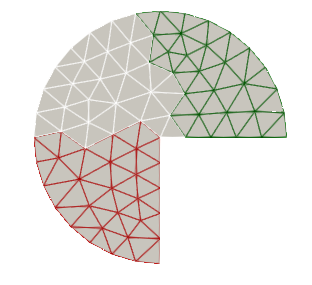
\includegraphics[scale=0.25]{Figures/Pacman}
			\end{figure}
		\end{minipage}
	\end{frame}
	\begin{frame}
		\frametitle{Mesh Refinement -- Adaptive Mesh Refinement: II}
		\begin{minipage}{0.75\textwidth}
			$\newline$
			\lstinputlisting[language=Python,firstline=92, lastline=106]{Codes/PacmanV2.py}
		\end{minipage}
		\begin{minipage}{0.15\textwidth}
			\vspace{-0.3cm}
			\begin{figure}
				\centering
				$\newline$
				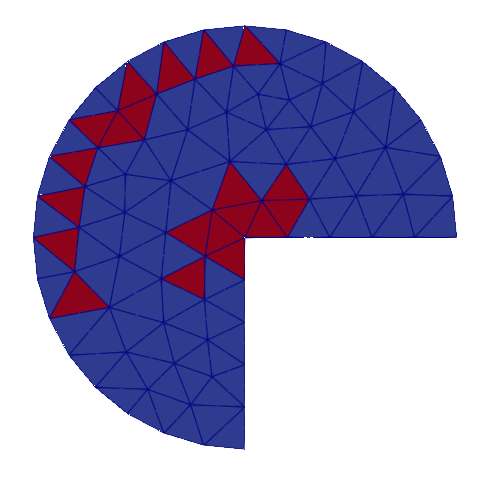
\includegraphics[scale=0.15]{Figures/PacmanMark}
				$\newline$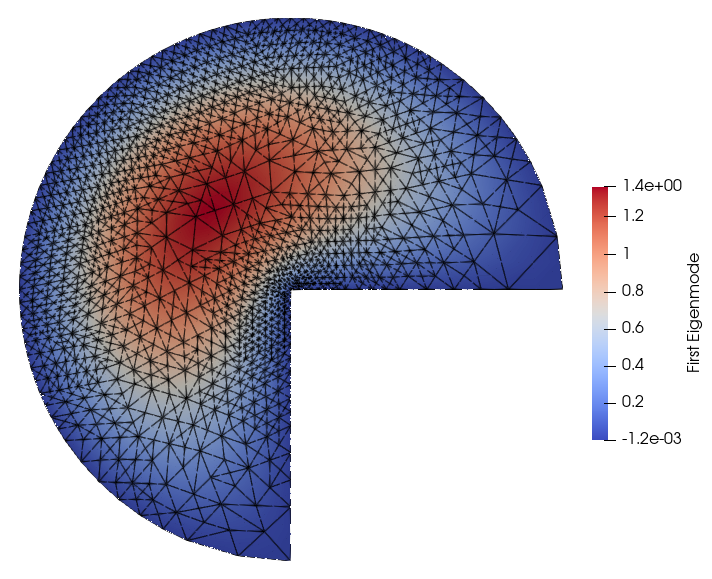
\includegraphics[scale=0.115]{Figures/PacmanAdp}
			\end{figure}
		\end{minipage}
	\end{frame}
	\begin{frame}
		\frametitle{Conclusion}
		$\newline$
		\begin{itemize}
			\item[\color{oxfordblue}$\blacktriangleright$] Mesh \textbf{hierarchy awareness}, using Firedrake \texttt{HierarchyBase} class.
			\item[\color{oxfordblue}$\blacktriangleright$] Make the implementation works in \textbf{complex} arithmetic.
			\item[\color{oxfordblue}$\blacktriangleright$] Support for \textbf{anisotropic} mesh refinement, using NetGen \texttt{ZRefinement} and \texttt{HPRefinement} methods.
			\item[\color{oxfordblue}$\blacktriangleright$] Support for NetGen \textbf{high order} mesh in Firedrake.
			\item[\color{oxfordblue}$\blacktriangleright$] Support for MFEM \textbf{GLVIS} mesh and solution live display, thanks to PETSc-GLVIS interface.
		\end{itemize}
	\end{frame}
\end{document}
